\documentclass[11pt]{article}
\usepackage[utf8]{inputenc}
\usepackage[T1]{fontenc}
\usepackage[brazil, english]{babel}
\usepackage{amsmath}
\usepackage{amsfonts}
\usepackage{graphicx}
\usepackage{setspace}
\usepackage{geometry}
\usepackage{indentfirst}
\usepackage[small,bf]{caption}

\begin{document}
\selectlanguage{brazil}
\begin{titlepage}
\begin{center}
\textsc{\Large Relatório Anual \\}
\textsc{\Huge Quebra de simetria espontânea,
              Limites Cognitivos e Complexidade
              de Sociedades}\\[0.5cm]
\vfill
\textsc{\small {\it Estudante:} \/Felippe Alves Pererira\\ 
               {\it Orientador:}\/Nestor Caticha\\
       }
\textsc{universidade de são paulo - instituto de física}\\
\textsc{\small departamento de física geral}\\
\small \today
\end{center}
\end{titlepage}

\newpage

\selectlanguage{brazil}

\newpage\null\thispagestyle{empty}\newpage
\section{Introdução}

Remontam aos primórdios do pensamento humano as questões sobre sua própria
natureza, em várias de suas manifestações. Dentre elas, aquelas sobre
o surgimento das sociedades e outras instituições de caráter cooperativo como
produto das interações entre pessoas têm sido objeto de estudo
nos últimos anos e têm mostrado resultados interessantes
\cite{CatichaetalA,Schonmannetal2011a,Perreault,Jonatas,visujeca}.

É dentro desse contexto que este projeto está inserido. Mais especificamente, o
objetivo do projeto é buscar novas perguntas e novo conhecimento sobre o
surgimento, estabilidade e coexistência de grupos com diferentes valores morais
e aplicar esse conhecimento no entendimento
da origem de crenças, pensamento religioso, ou instituições religiosas.

Para esse fim, é preciso formular perguntas, e modelos para responder estas
perguntas, que possibilitam verificar a existência de uma
instituição, grupo ou organização, a partir da interação entre indivíduos ao
longo do tempo. É necessário também entender o mecanismo de interação e
sua relação com cada indivíduo. A seguir, uma abordagem mais detalhada da
estratégia usada neste projeto para atacar o problema proposto.

\subsection{Teoria dos Fundamentos Morais e Modelos de Agentes}

A Teoria dos Fundamentos Morais, proposta pelo psicólogo social {\it J.
Haidt} \cite{Haidt}, traz duas características importantes para a compreensão
da moralidade humana. A primeira é que os julgamentos morais ocorrem de forma
espontânea e (para todos os efeitos imediata) quando uma pessoa é exposta a uma
questão de cunho moral. Isso significa que não há tempo para o raciocínio
interfirir na consequência dessa exposição, ou que toda racionalização
acontece após tal consequência. A segunda diz respeito a caracterização das
bases morais. Segundo {\it Haidt}, ao menos $5$ bases morais são relevantes,
sendo elas:
\begin{enumerate}
    \item Violência / Cuidado
    \item Justiça / Trapaça
    \item Lealdade ao grupo / Traição
    \item Respeito à autoridade / Subversão
    \item Santidade (ou Pureza) / Degradação
\end{enumerate}

Essas duas características são importantes pois possibilitam a elaboração de
modelos de agentes caracterizados por um vetor em $5$ dimensões
que determina
sua matriz moral, nos quais é possível estabelecer uma interação instantânea.
Isso permite que os agentes possam viver
uma dinâmica onde suas opiniões dependem de um aprendizado prévio (ou em curso)
e que permita a emergência de coletividade no campo das opiniões.

\subsection{O Modelo}

\newcommand{\w}[1]{%
    \ensuremath{\displaystyle%
        \bold{w}_{#1}        
    }
}

\newcommand{\zt}{%
    \ensuremath{\displaystyle%
        \bold{z}        
    }
}

\newcommand{\ip}[2]{%
    \ensuremath{\displaystyle%
        {#1} \cdot {#2}
    }
}

\newcommand{\inp}[1]{\ensuremath{\displaystyle%
    \left(#1\right)}}

\newcommand{\ina}[1]{\ensuremath{\displaystyle%
    \left<#1\right>}}

\newcommand{\ins}[1]{\ensuremath{\displaystyle%
    \left[#1\right]}}

\newcommand{\inc}[1]{\ensuremath{\displaystyle%
    \left{#1\right}}}

No espírito de formular perguntas em cima da plataforma estabelecida pela Teoria
dos Fundamentos Morais e da ideia de modelos de agentes, é proposto um modelo
básico, do qual variações simples permitem o teste de diferentes hipóteses. Esse
modelo deve capturar as características destacadas acima e permitir o uso de
técnicas bem estabelecidas, como os métodos da mecânica estatística e teoria do
aprendizado de máquina.

Considere um sistema formado por $N$ agentes, sendo cada um deles caracterizado
por um vetor $\w{i} \in \mathbb{R}^D$, com $i \in \{1,\ldots,N\} = \mathcal{V}$
e $|\w{i}|=1$ para todo $i$.
Os vetores $\w{i}$ representam a matriz moral de cada agente, na qual reside as
bases de suas opiniões (definidas adiante).

Esses agentes estão dispostos numa rede social de interações
caracterizada pelo grafo $\mathcal{G}=(\mathcal{V},\mathcal{E})$, onde 
$\mathcal{V} = \{1,\ldots,N\}$, conjunto dos índices dos agentes, são os 
vértices e $E$ as arestas do grafo, do qual um elemento é denotado por
$(ij)$ quando os agentes $i$ e $j$ interagem (são primeiros vizinhos no grafo).

Seja, também, $\bold{x}^{\mu} \in \mathbb{R}^D$, com $\mu \in \{1,\ldots,P\}$
e $|\bold{x}^{\mu}|=1$ para todo $\mu$, um conjunto de questões morais às quais
os agentes serão expostos.
A opinião de um agente $i$ sobre uma questão $\mu$ é definida pelo produto
escalar dos vetores $h_i^{\mu}=\ip{\w{i}}{\bold{x}^{\mu}}$.
O lado ou a postura desse agente com relação a essa questão é dada pelo sinal
da opinião $\sigma_i^{\mu}=\mathrm{sgn}(h_i^{\mu})$.

Essa base permite o uso dos resultados da teoria de aprendizado supervisionado
para uma rede neural de uma camada. Tal situação demanda uma rede aluno e uma
rede professor e mostra que, dado um número suficientemente grande de exemplos,
caso as redes aluno e professor tenham a mesma dimensão, então a rede aluno
consegue imitar a rede professor.
Cada exemplo é composto por um vetor questão e uma resposta dada pelo sinal do
produto escalar do vetor professor com o vetor questão.
Além disso, é possível mostrar \cite{Engel} que essa dinâmica de
aprendizado pode ser vista como a descida pelo gradiente de um potencial de
interação entre aluno e professor.

Seguindo o modelo proposto em \cite{visujeca}, considere o cenário em que
um par de agentes, $(ij)$ interage através da troca de opiniões a respeito de 
uma questão moral. Digamos que, no instante $t$, o agente $i$ é o aluno e $j$ o
professor, de modo que o exemplo recebido por $i$ é \inp{\bold{x}^{\mu},
\sigma_j^{\mu}}.
Então o agente $i$ atualiza sua matriz moral da seguinte forma:

\begin{equation*}
    \w{i}(t+1)=\w{i}(t)+\eta\bold{\nabla}_j V_{\delta}(h_i^{\mu}(t)h_j^{\mu}(t))
\end{equation*}

com $\bold{\nabla}_j = \sum_{k=1}^D \bold{e}^k\frac{\partial}{\partial w_j^k}$
é o operador gradiente relativo às componentes de \w{j} e o potencial de 
interação entre agentes é dado por

\begin{equation}
    V_{\delta}(h_i^{\mu}h_j^{\mu})=-\frac{1+\delta}{2}h_i^{\mu}h_j^{\mu}+
    \frac{1-\delta}{2}|h_i^{\mu}h_j^{\mu}|
\end{equation}

onde $\delta$ foi mostrado estar relacionado com o tipo de aprendizado e
ideologia política do agente \cite{Jonatas}. 
O gráfico do potencial $V_{\delta}$ pode ser visto no quadro à esquerda na
figura~\ref{figV}

\begin{figure}[h!]
  \centering
      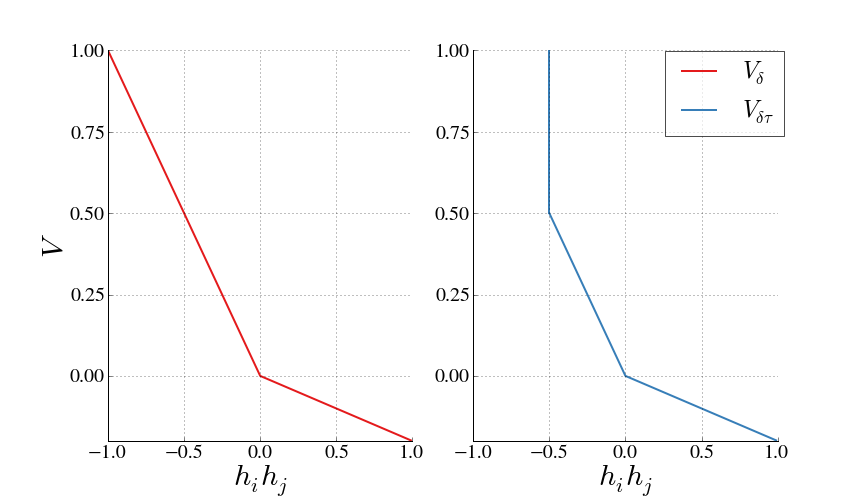
\includegraphics[width=1.0\textwidth]{V.png}
  \caption{Gráfico do potencial de interação entre agentes em função da 
  concordância/discordância entre os agentes $(ij)$. À esquerda o potencial
  $V_{\delta}$ e à direita o potencial $V_{\delta \tau}$, ambos construídos
  com $\delta = 0.2$ e o último construído com $\tau = 0.5$.}
    \label{figV}
\end{figure}


\subsection{Busca por Consenso}

A primeira tarefa foi recuperar os resultados que caracterizam o
surgimento de consenso num cenário simples \cite{visujeca, Jonatas}.
Considere o caso em
que a sociedade debate apenas um assunto, ou seja $P=1$ e $\bold{x}^{\mu} =
\bold{x}^1 = \zt$.
Seguindo \cite{CaVi},chamemos esse assunto de {\it zeitgeist}, e suponhamos que
ele representa um sumário dos assuntos importantes para a tal sociedade. Neste
cenário temos $h_i = \ip{\w{i}}{\zt}$ representando a opinião do agente $i$
sobre o zeitgeist e podemos observar a formação de consenso através da média de 
$h_i$ na sociedade.

Para isso, usando os métodos da mecânica estatística, obtemos que a distribuição
de probabilidades para o estado da sociedade, representado pelo conjunto
dos vetores $\w{i}$, é dado pela distribuição de Boltzmann

\[P\inp{\underline{\w{}}}=\frac{1}{Z}\mathrm{e}^{\beta \mathcal{H}}\]

com $\mathcal{H}=\sum_{(ij)} V_{\delta}(h_ih_j)$ e $\beta$, o multiplicador de
Lagrange do vínculo que fixa do valor esperado de $\mathcal{H}$, interpretado
como uma medida da pressão social.

Através de simulações de Monte Carlo para esse sistema foi possível construir as
curvas de "magnetização", ou neste caso de opinião, para o sistema, resultado
mostrado na figura~\ref{m-b-d}

\begin{figure}[h!]
  \centering
      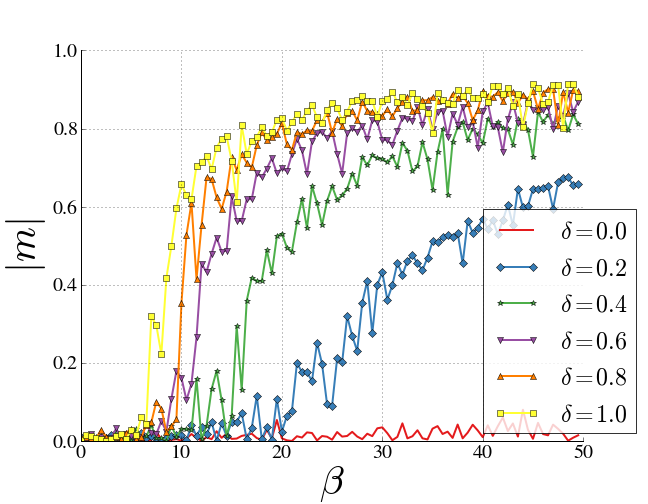
\includegraphics[width=1.0\textwidth]{mbd.png}
  \caption{Gráfico da média das opiniões $m=\left<h\right>$ pela pressão social
      $\beta$ para diferentes valores do estilo cognitivo $\delta$}
    \label{m-b-d}
\end{figure}

A análise da figura mostra que o parâmetro $\delta$ possibilita o surgimento de
consenso na sociedade desde que seu valor seja diferente de zero e que haja
suficiente pressão social. Mais que isso, as curva de opinião são similares às
curvas de magnetização que caracterizam a transição de fases do modelo de Ising.


\subsection{Impedindo o Consenso Global}

Como consequência do resultado para o consenso da sociedade, fica evidente que
esse modelo não suporta a manutenção de diferentes opiniões em situações de alta
pressão social. Em analogia com sistemas magnéticos, não é possível a
coexistência de regiões de diferentes magnetizações. 
Uma vez que tal coexistência é interessante para avaliar a tolerância a
diferentes opiniões, uma forma de contornar essa limitação é necessária.

A primeira tentativa nessa direção foi barrar o aprendizado no caso de extrema
discordância. Isso pode ser feito introduzindo um corte no potencial para
valores de concordância/discordância, $h_i h_j$, negativos e com grande módulo.
Se chamarmos o ponto onde o corte é feito de $-\tau$, o potencial de interação
será

\newcommand{\ag}{%
    \ensuremath{\displaystyle%
        h_ih_j
    }
}

\newcommand{\dpos}{%
    \ensuremath{\displaystyle%
        \frac{1+\delta}{2}
    }
}

\newcommand{\dneg}{%
    \ensuremath{\displaystyle%
        \frac{1-\delta}{2}
    }
}

\[V_{\delta \tau}=
    \begin{cases}
        -\dpos \ag + \dneg |\ag| & \text{, se } \ag \geq -\tau \\
        \infty & \text{, se } \ag < -\tau
    \end{cases}
\]

Note que esse, para $\tau = 1$, esse potencial se reduz a $V_{\delta}$, pois o
parâmetro de concordância/discordância, $h_ih_j$, pode assumir valores apenas
entre $-1$ e $1$. O papel de $\tau$ é representar a confiança na opinião de
acordo com o quão 'absurdo' um agente pode atribuir à opinião de outro. 
Portanto, parece razoável dar o nome de confiança as parâmetro $\tau$.

Novamente, simulações de Monte Carlo foram feitas para analisar as curvas de
opinião e avaliar as condições em que há surgimento de consenso.
Os resultados estão na figura~\ref{data1}.
Como é possível notar, a habilidade de ignorar opiniões nas quais não há
confiança é suficiente para possibilitar o surgimento de polarização em torno do
zeitgeist. Para ver que este é o caso, note que, pra $\tau=0.1$, não há consenso
e, a baixa pressão social, $\beta$, o histograma de similaridade entre agentes,
$\rho_{ij} = \ip{\w{i}}{\w{j}}$ é unimodal e centrado em zero e com alta
dispersão.
Isso significa que as opiniões dos agentes assumem todos os possíveis valores
entre $-1$ e $1$.
A alta pressão social, porém, o histograma tem duas modas: $-1$ e $1$ e com
menos dispersão em torno de cada uma delas, o que implica que existem apenas
valores de opinião próximos das modas.
Em contraposição, a situação com $\tau=0.9$ e alta pressão social tem apenas uma
moda, $1$ ou $-1$.

\begin{figure}[h!]
  \centering
      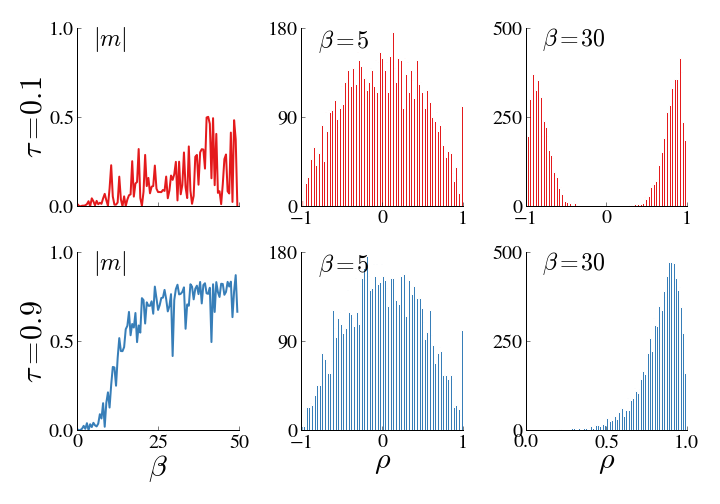
\includegraphics[width=1.0\textwidth]{data1.png}
  \caption{Resultados para o modelo com confiança e reputação.
  Cada linha tem gráficos construídos com o valor fixo para $\delta=0.8$ e
  valores de $\tau$ iguais a $0.1$ para a linha de cima e $0.9$ para a de baixo.
  Os gráficos da coluna à esquerda são as curvas de opinião, os demais são os
  histogramas da similaridade entre agentes $\rho_{ij} = \ip{\w{i}}{\w{j}}$}
  \label{data1}
\end{figure}


\subsection{Busca por Reputação}

Outra caraterística interessante de instituições religiosas e associações morais
é a notoriedade e influência de figuras ilustres e popularmente respeitadas,
comi sacerdotes ou personalidades formadoras de opinião. Isso significa que um
modelo adequado para entender esse fenômeno deve ser capaz de atribuir maior
peso para a opiniões de indivíduos com mais notoriedade.

Para atacar esse problema foi introduzida ao modelo uma dinâmica para as
relações entre indivíduos. Essa dinâmica possibilita que a interação entre dois
agentes seja fortalecida conforme eles concordem ou enfraquecida quando
discordam e que eles tenham um método de escolher com qual agente querem
interagir baseado na força da relação. Especificamente, foi atribuído um campo
$R_{ij}$ a cada aresta $(ij) \in E$ representando a reputação atribuída ao
agente $i$ pelo agente $j$. A probabilidade do agente $i$ ser escolhido pelo
agente $j$ para trocar informação em um dado momento depende de $R_{ij}$, que
cresce de acordo com a concordância entre os agentes cada vez que interagem.

A evolução da reputação que o agente $i$ atribui ao agente $j$ é descrita pela
seguinte equação

\[R_{ij}(t+1) = R_{ij}(t) + \epsilon h_i(t)h_j(t)\]

toda vez que o agente $j$ for escolhido por $i$ para interagir, cuja
probabilidade é dada por 

\[p_{ij} = \frac{R_{ij}-R_{min}}{\sum_k \inp{R_{ik}-R_{min}}}\]

com $R_{min}(t)=\mathrm{min}_k(R_{ik}(t))$

Mais uma vez, simulações de Monte Carlo foram realizadas para verificar as
consequências, dessa vez na estrutura social, resultados mostrados na
figura~\ref{data2}
Inicialmente, a sociedade era totalmente conectada, todos os agentes se
relacionavam de uniforme. Tal situação é representada por um grafo completo. Com
a evolução da reputação, grupos de opinião similar apareceram apenas quando
polarização era possível. 
Ou seja, para baixo valor de confiança, segregação social por escolhas morais
pode surgir, desde que os agentes possam dar preferência para agentes que os
"agradem" mais. Porém, isso não é o bastante para o surgimento de um agente mais
influente dentre dos grupos.

\begin{figure}[h!]
  \centering
      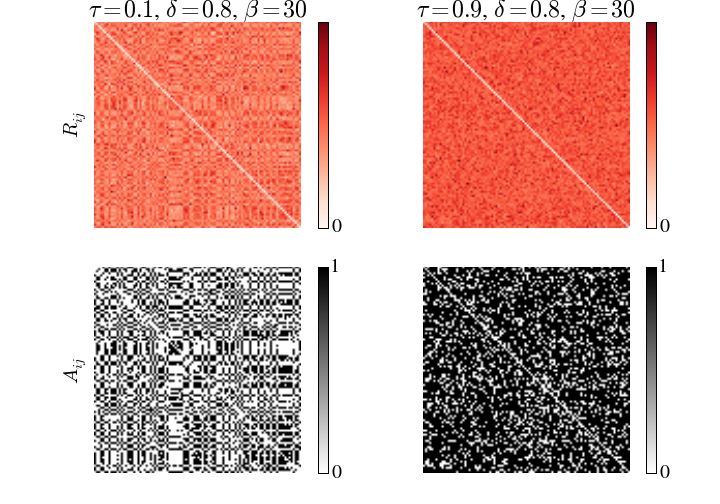
\includegraphics[width=1.0\textwidth]{data2.png}
  \caption{Fotografias das estrutura social induzida pela reputação. A linha de
  cima mostra matrizes da reputação de cada agente distintas apenas no valor de
  confiança. A linha de baixo é a estrutura social induzida, ou seja, a matriz
  de adjacência}
  \label{data2}
\end{figure}

\section{Sumário dos avanços obtidos}

Até então, foram estudados separadamente cada característica do fenômeno em foco,
além de algumas tentativas de uni-los num mesmo modelo. Embora a perspectiva
global ainda esteja fragmentada, nos próximos meses, espera-se, será possível
unir os resultados atuis numa compreensão mais concreta do fenômeno estudado.
Além disso, mais esforço será dedicado à obtenção de resultados no objetivo de
caracterizar agentes formadores de opinião.

Além da busca pela estruturação, alguns resultados recentes trazem possíveis
bases experimentais para o teste dos modelos \cite{Toorn} e
uma ampla base de dados pode fornecer diferentes perspectivas de
análise e, com sorte, dar suporte a previsões do modelo.\footnote{Uma base de
dados promissora é o atlas etnográfico de George P. Murdock, que pode ser
encontrado online em http://eclectic.ss.uci.edu/~drwhite/worldcul/atlas.htm}


\begin{thebibliography}{99}

\bibitem{Jaynes}E. T. Jaynes {\it Probability theory: The Logic of
    Science} \/Cambridge University Press, Cambridge (2003)

\bibitem{Ariel} A. Caticha Lecture Notes on information Theory,

\bibitem{mackay} MacKay D.J.C., \textit{Information Theory, Inference
    and Learning Algorithms}
Cambridge University Press, Cambridge, (2003).

\bibitem{Parisi} G. Parisi {\it et al, Spin Glasses and Beyond}

\bibitem{Engel} A. Engel and C. van den Broeck {\it Statistical
    Mechanics of Learning}

\bibitem{Nishimori} Nishimori, Statistical Physics of Spin Glasses and Information Processing: An Introduction

\bibitem{Ostrom}Ostrom, Elinor (1990). Governing the Commons: The Evolution of Institutions for Collective Action. Cambridge University Press. ISBN 0-521-40599-8; Ostrom, Elinor (July 2009). "A General Framework for Analyzing Sustainability of Social-Ecological Systems". Science 325: 419–422.

\bibitem{Hardin}Garrett Hardin
"The Tragedy of the Commons". Science 162 (3859): 1243–1248. 1968.

\bibitem{Strandburg}Michael J. Madison, Brett M. Frischmann
and Katherine J. Strandburg,
Legal Studies Research Paper Series
Working Paper No. 2008-26
August 2008

\bibitem{Estes}William K. Estes, Research and Theory on the
Learning of Probabilities,
Journal of the American Statistical Association, Vol. 67, No. 337
(Mar., 1972), pp. 81-102

\bibitem{CaVi}N.Caticha and R.Vicente ¨Agent-based social psycology: from neurocognitive processes to social data¨ Volume: 14, Issue: 5(2011) pp.711-731 Advances in Complex Systems (ACS)

\bibitem{Settle2010a}Settle, Jaime E Dawes, Christofer T Christakis, Nicholas A Fowler, James H (2010) 72,4 1189 ¨Friendships Moderates an Association Between a Dopamine Gene and Political Ideology.¨ The journal of politicsz

\bibitem{Kandel} Kandel, et al, Essentials of neural sciences and behavior.


\bibitem{Dunbar} R. Dunbar,  Grooming, Gossip, and the
Evolution of Language. Faber, London (1997)

\bibitem{Eisenberger} Eisenberger, N., Lieberman, M., and Williams, K., Does rejection hurt? An fMRI
study of social exclusion, Science 302 (2003) 290-292.

\bibitem{Mazur} Allan Mazur,
Biosociology
of Dominance
and Deference
ROWMAN and LITTLEFIELD PUBLISHERS, INC.
(2005

 \bibitem{Pumain}
Hierarchy in Natural
and Social Sciences
edited by
Denise Pumain, Springer (2006)

\bibitem{Bohem}Christopher Boehm
Hierarchy in the Forest
The Evolution of
Egalitarian Behavior, Harvard University Press (2001)

\bibitem{Earle} Timothy Earle,
How Chiefs came to power, Stanford University Press (1997)

\bibitem{Salzman} Philip Carl Salzman, Pastoralists: Equality, Hierarchy and
the State. Westview Press (2004)

\bibitem{Fleagle}Edited by
John G. Fleagle
Charles H. Janson
Kaye E. Reed, Primate Communities
Cambridge University Press (2004)

\bibitem{Wason} Paul K. Wason, The archaeology of rank
Cambridge University Press (1994)

\bibitem{Sassaman} Kenneth E. Sassaman, Journal of Archaeological Research Vol 12 september 2004

\bibitem{Menger} Carl Menger
On the Origins of Money
Economic Journal, volume 2,(1892) p. 239-55.
translated by C.A. Foley

\bibitem{Maisels}Charles Keith Maisels, The Emergence of
Civilization:
From hunting and gathering to
agriculture, cities, and the state in the
Near East,
Routledge   (2005)

\bibitem{CatichaetalA} N. Caticha, R. Calsaverini, R. Vicente, {\it
Cognitive limits and Breakdown of the Egalitarian Society} \/preprint (2012)

\bibitem{Schonmannetal2011a} R. Schonmann, R. Vicente e N. Caticha
Two-level Fisher-Wright framework with selection and migration: An approach to
studying evolution in group structured populations\.
arXiv:1106.4783 (2011)

\bibitem{Perreault}C. Perreault, C. Moya, and R. Boyd. A Baysian approach to the evolution of social learning. Evolution and Human Behavior, Proofs posted online April 2012

\bibitem{Jonatas}
Jônatas Eduardo da Silva César. Mecânica Estatística de Sistemas de Agentes
Baysianos: Aplicação à Teoria dos Fundamentos Morais. Tese defendida em 2014

\bibitem{visujeca} R. Vicente, A. Susemihl, J.P. Jericó, N. Caticha. Moral
    foundations in an interacting neural networks society

\bibitem{Toorn}Jojanneke van der Toorn, Jaime L. Napier and John F. Dovidio. We the People: Intergroup Interdependence Breeds Liberalism
Social Psychological and Personality Science published online 5 December 2013

\bibitem{Haidt} Graham, Jesse; Haidt, Jonathan; Nosek, Brian A.
    Liberals and conservatives rely on different sets of moral foundations.
Journal of Personality and Social Psychology, Vol 96(5), May 2009, 1029-1046

\end{thebibliography}

\end{document}


